\chapter{Primer in financial data}
\label{chapterIntroFinDat}
Although financial data comes in many shapes and forms, this work will be 
centered around the one that comes from stocks or indices (basket of 
financial instruments). To make matters easier, instead of thinking of 
financial instruments one can think about the underlying price time series.
\\

That is why it is important to introduce the time series $\{ p_t \}$, which 
is the price of the stock/index at the discrete time stamp $t$. Note that $t$ 
will will depend on the sampling frequency used to gather data.\\

\textbf{Frequency:}
\begin{itemize}
	\item Low Frequency Data (LF): Daily, Monthly, Quarterly.
	\item High Frequency Data (HF): Intraday (30 min., 5 min. \ldots)
\end{itemize}

\vspace{.4cm}

Having introduced these concepts, it should be pointed out that modeling in 
finance is carried out with the natural logarithm of the price (log-prices) 
instead of regular prices. It will be referred to as $y_t := \log (p_t)$. To 
illustrate this, the simple model, yet widely used, of a random walk with 
drift will be introduced:

\begin{equation*}
	y_t = y_{t - 1} + \mu + \epsilon_t	
\end{equation*}

where $\epsilon_t \sim \text{ i.i.d. } N(0, \sigma^2)$

\section{Asset returns}
The next concept to introduce are the returns, which is a technique to 
normalize prices. To be specific, it allows comparison between different 
time series regardless of the price value. The two types that are going to 
be used are the linear and logarithmic returns.

\begin{itemize}
	\item \textbf{Linear:} $R_t(1) \equiv R_t := \frac{p_t - p_{t-1}}
	{p_{t - 1}} = \frac{p_t}{p_{t - 1}} - 1$
	\item \textbf{Logarithmic:} 
	$r_t(1) \equiv r_t := \log \left( \frac{p_t}{p_{t-1}} \right) = 
	\log (p_t) - \log (p_{t - 1}) = y_t - y_{t - 1}$
\end{itemize}
Where $\log$ is the natural logarithm.\\

A few properties that can be highlighted:
\begin{enumerate}
	\item $r_t = \log (1 + R_t)$
	
	\item The Taylor series of $\log (1 + x) = \sum_{k = 1}^{\infty} 
	(-1)^{k + 1} \frac{x^k}{k}$ yields $r_t \approx R_t$ 	whenever 
	$R_t \approx 0$
	
	\item Compounded linear returns:\\
	$R_t(k) := \frac{p_t - p_{t-k}}{p_{t-k}} = \frac{p_t}{p_{t-k}} - 1 = 
	\frac{p_t}{p_{t-1}} \ldots \frac{p_{t-(k-1)}}{p_{t-k}} - 1 = 
	(1 + R_t) \cdot 	(1 + R_{t-1}) \ldots (1 + R_{t-(k-1)}) - 1$
	
	\item Compounded log-returns:\\
	$r_t(k) := \log \left( \frac{p_t}{p_{t-k}} \right) = y_t - y_{t-k} = 
	(y_t - y_{t-1}) + \ldots + (y_{t-(k-1)} - y_{t-k}) = 
	r_t + \ldots + r_{t-(k-1)}$
\end{enumerate}

\vspace{.2cm}

With the purpose of displaying what has been defined, in figures 
\ref{fig:logReturnsSP500} and \ref{fig:logPricesSP500} the log-returns and 
log-prices of the S\&P500 have been plotted for the period that spans from 
2015-01-01 to 2018-10-01.\\

Regarding the variation of returns, and hence the variation of prices, the 
term \textbf{volatility} comes into play. It will be denoted as 
$\sigma := \sqrt{ \mathbb{E} [ (r_t - \mathbb{E} [r_t] )^2 ] }$, 
which is the standard deviation of log-returns.

\begin{figure}[htbp]
\centering
	\begin{minipage}{.5\textwidth}
		\centering
		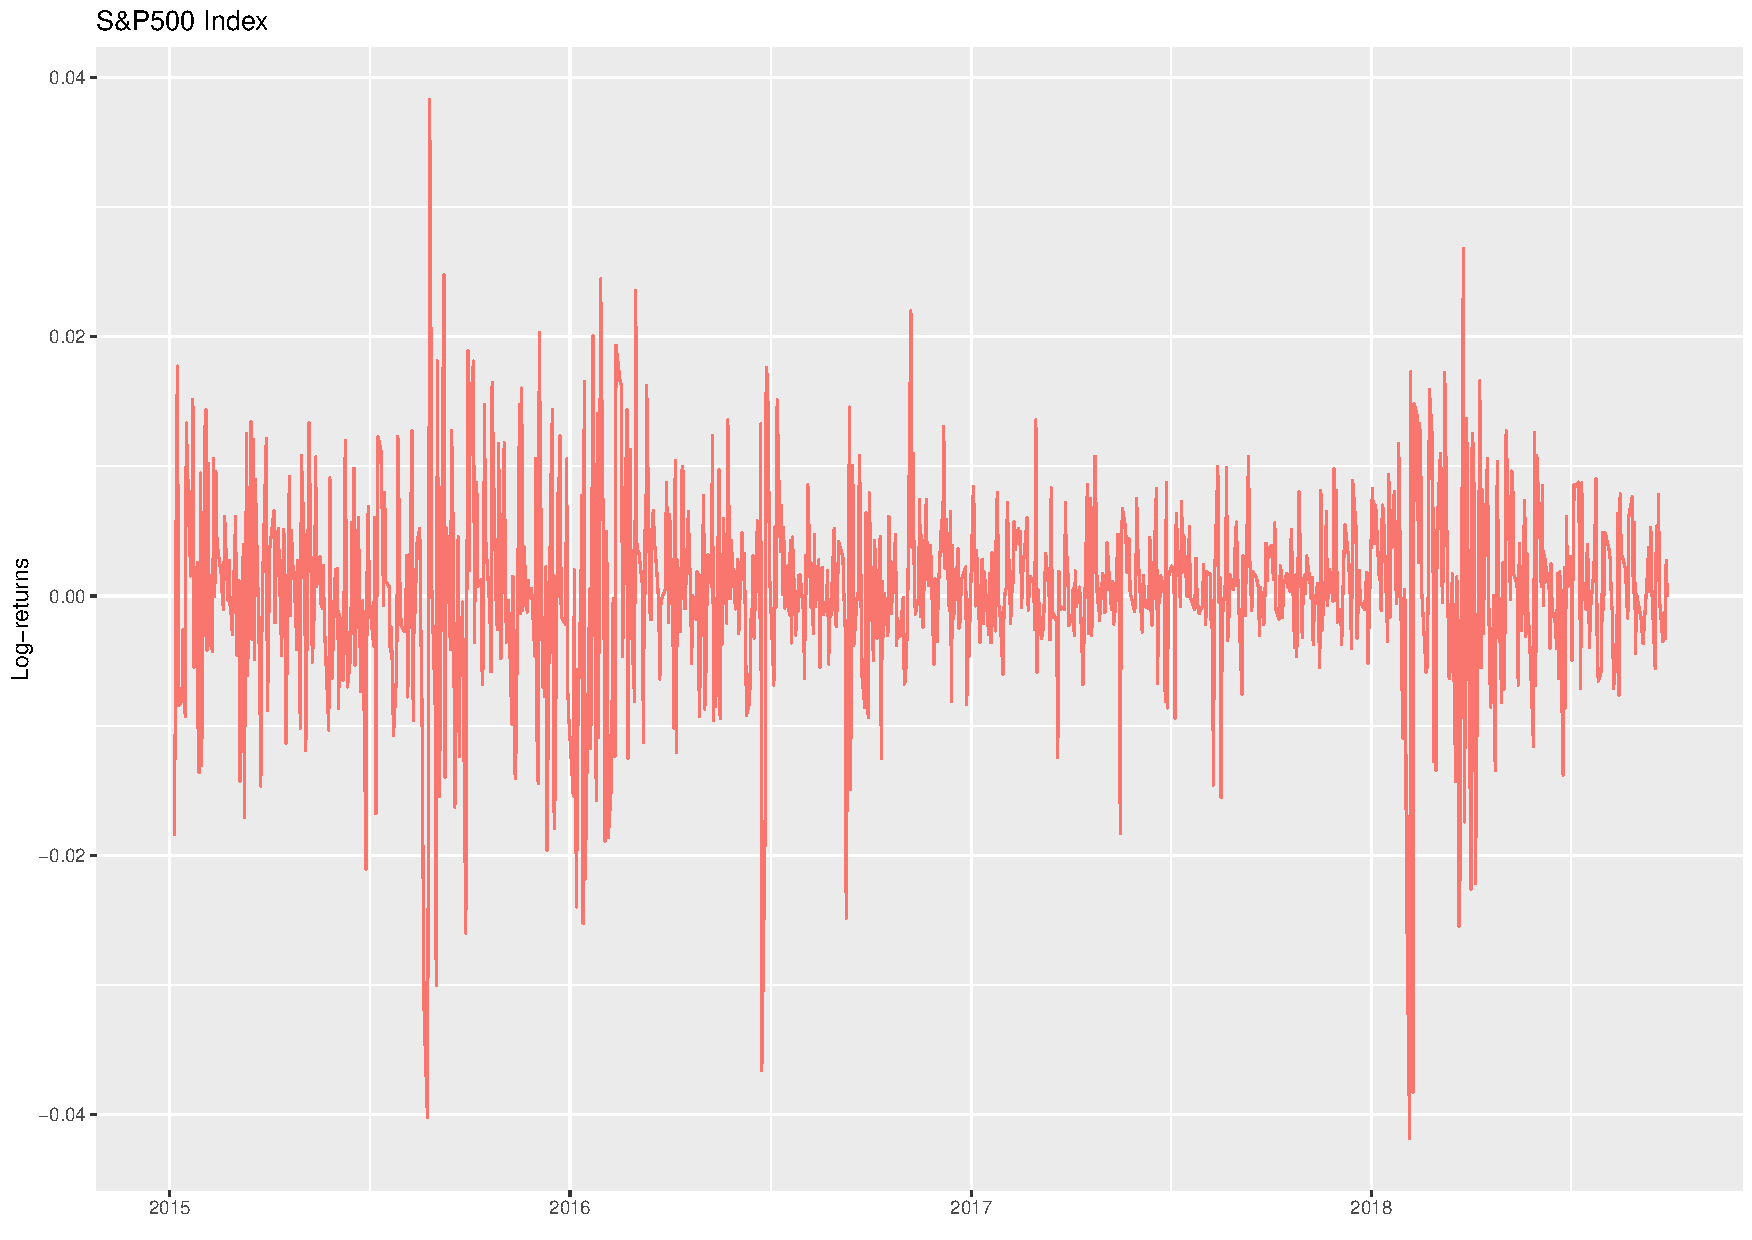
\includegraphics[scale=.25]{img/finData/logReturns}
		\caption{Log-Returns of the S\&P500}
		\label{fig:logReturnsSP500}
	\end{minipage}%
	\begin{minipage}{.5\textwidth}
		\centering
		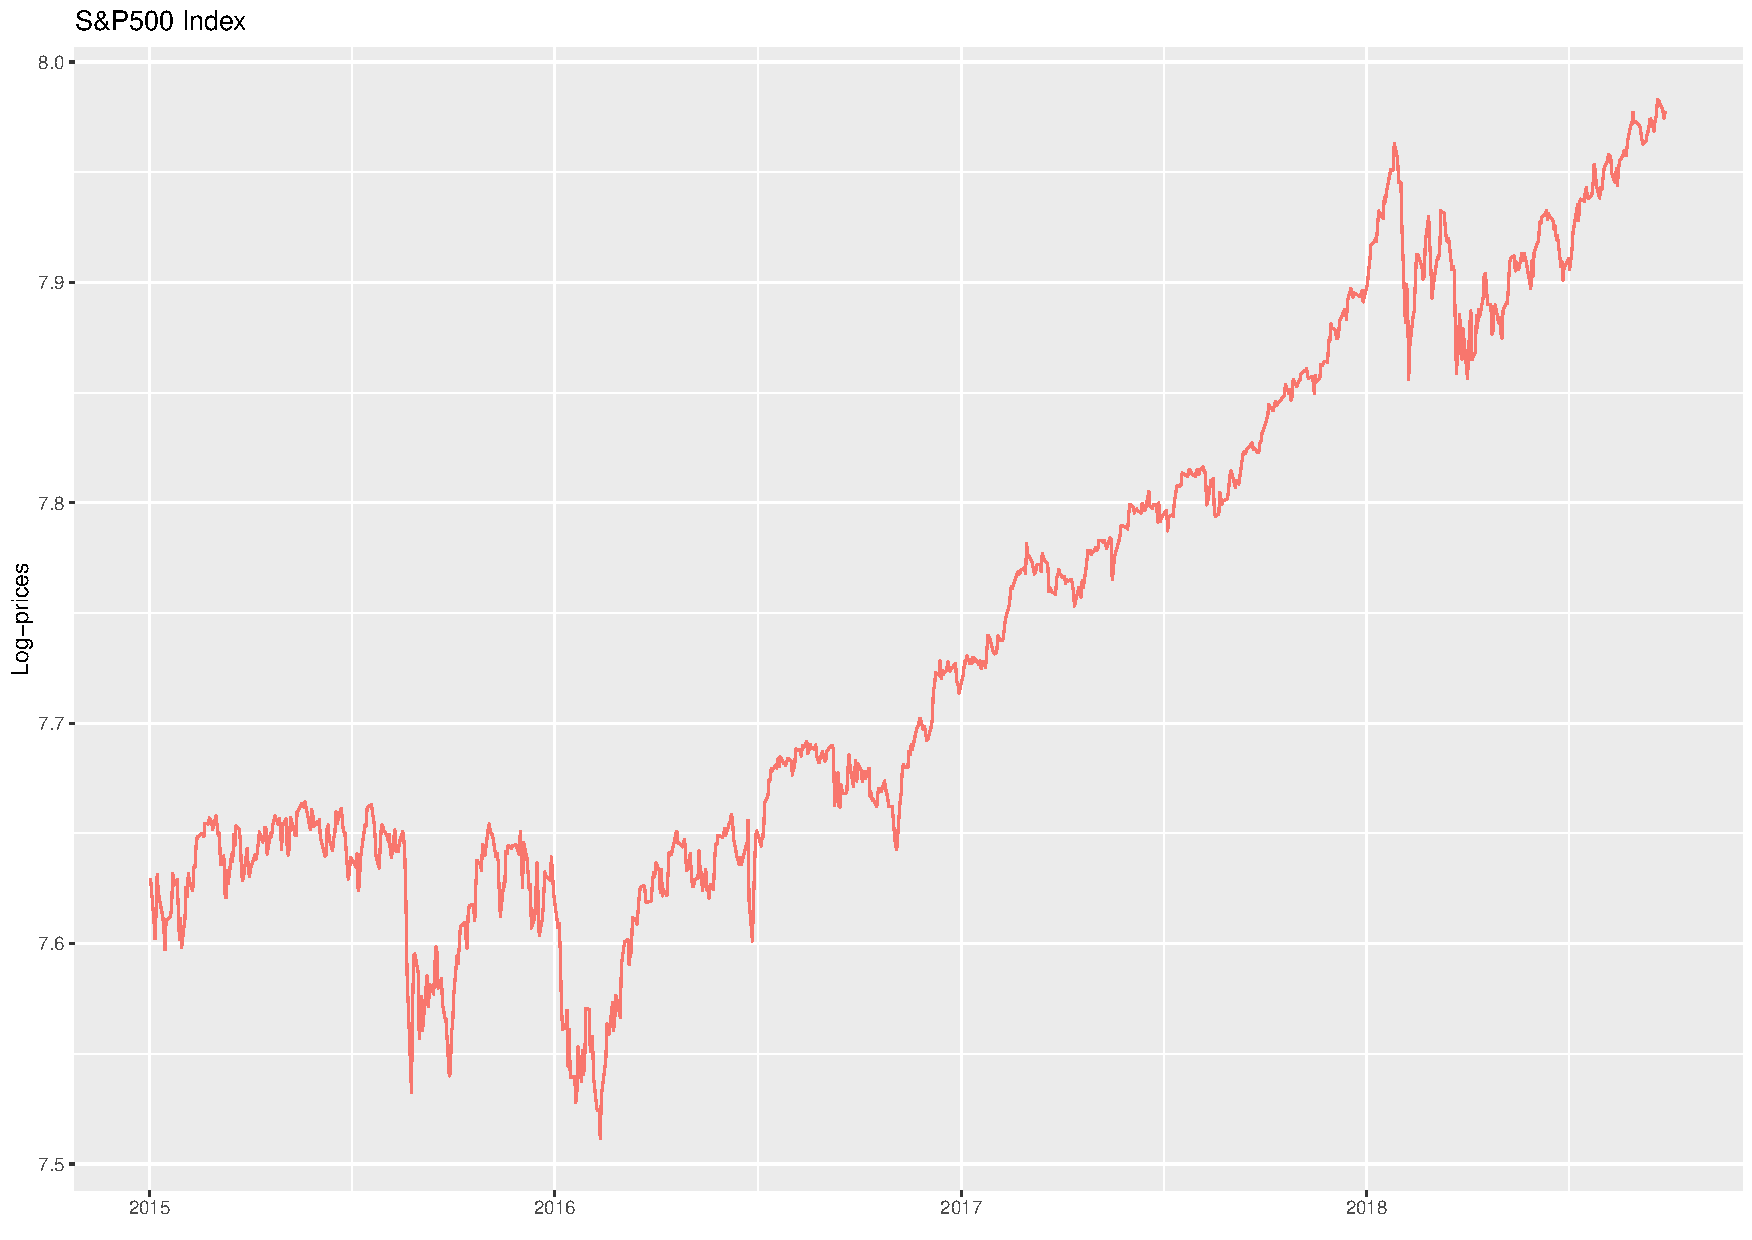
\includegraphics[scale=.25]{img/finData/logPrices}
		\caption{Log-Prices of the S\&P500}
		\label{fig:logPricesSP500}
	\end{minipage}
\end{figure}

\section{Stylized facts}
\label{sec:stylizedFacts}
In an attempt to portray financial data without the need of a theoretical 
framework, Rama Cont presents financial data in~\cite{stylizedFacts}. To 
introduce empirical properties he uses stylized facts, which are 
broad generalizations that summarize data.\\

In other words, this section will serve as a brief introduction to 
properties of financial data which have been observed in various types of 
financial markets. However, bear in mind that this is a first approximation 
and that stylized facts are not by any means facts.\\

With that being said, the stylized facts relevant to this work presented 
in~\cite{stylizedFacts} are:

\begin{enumerate}
	\item \textbf{Absence of autocorrelations:} linear autocorrelations of 
	asset returns are insignificant, except for small intraday scales. See 
	figure \ref{fig:acfDailyLogRet} for the autocorrelations of daily 
	S\&P500 log-returns.
	
	\item \textbf{Heavy tails:} The pdf of returns is heavy-tailed. That is, 
	its tails fall much slower than a Normal pdf, which falls exponentially 
	to zero.
	
	\item \textbf{Gain/loss asymmetry:} Extreme down movements are far more 
	common than huge upswings.
	
	\item \textbf{Aggregational Gaussianity:} The probability density 
	function (pdf) of log-returns approaches the one of a Gaussian random 
	variable as one increases the time scale over which returns are 
	calculated (see figure \ref{fig:HistLogRet}).
	
	\item \textbf{Intermittency:} Regardless of the time scale, returns 
	display high variability.
	
	\item \textbf{Volatility clustering:} As it can be seen in figure 
	\ref{fig:logReturnsSP500}, high volatility (dispersion of log-returns) 
	events tend to come in clusters.
\end{enumerate}


%\cite{stylizedFacts, AdvFML}

\section{Statistical properties}
In figure \ref{fig:acfDailyLogRet} one can see the autocorrelations of daily 
log-returns. The definition, as in~\cite{acfDefinition}, of the 
log-returns autocorrelation of lag $k$ is the following:

\begin{equation*}
	\rho_k = \frac{\text{Cov}(r_t, r_{t + k})}{\sqrt{\text{Var} [r_t]}
	\sqrt{\text{Var} [r_{t + k}]}}
\end{equation*} 

Where $\text{Cov}(r_t, r_{t + k})$ is the covariance of $r_t$ and 
$r_{t + k}$ and $\text{Var}[r_t]$ the variance of $r_t$.\\

It can be seen that, by definition, $\rho_0 = 1$. Apart from that, the rest 
of lags are insignificant or barely surpass the significant threshold 
(dotted line). This confirms the first stylized fact presented in section 
\ref{sec:stylizedFacts}.

\begin{figure}[hbtp]
	\centering
	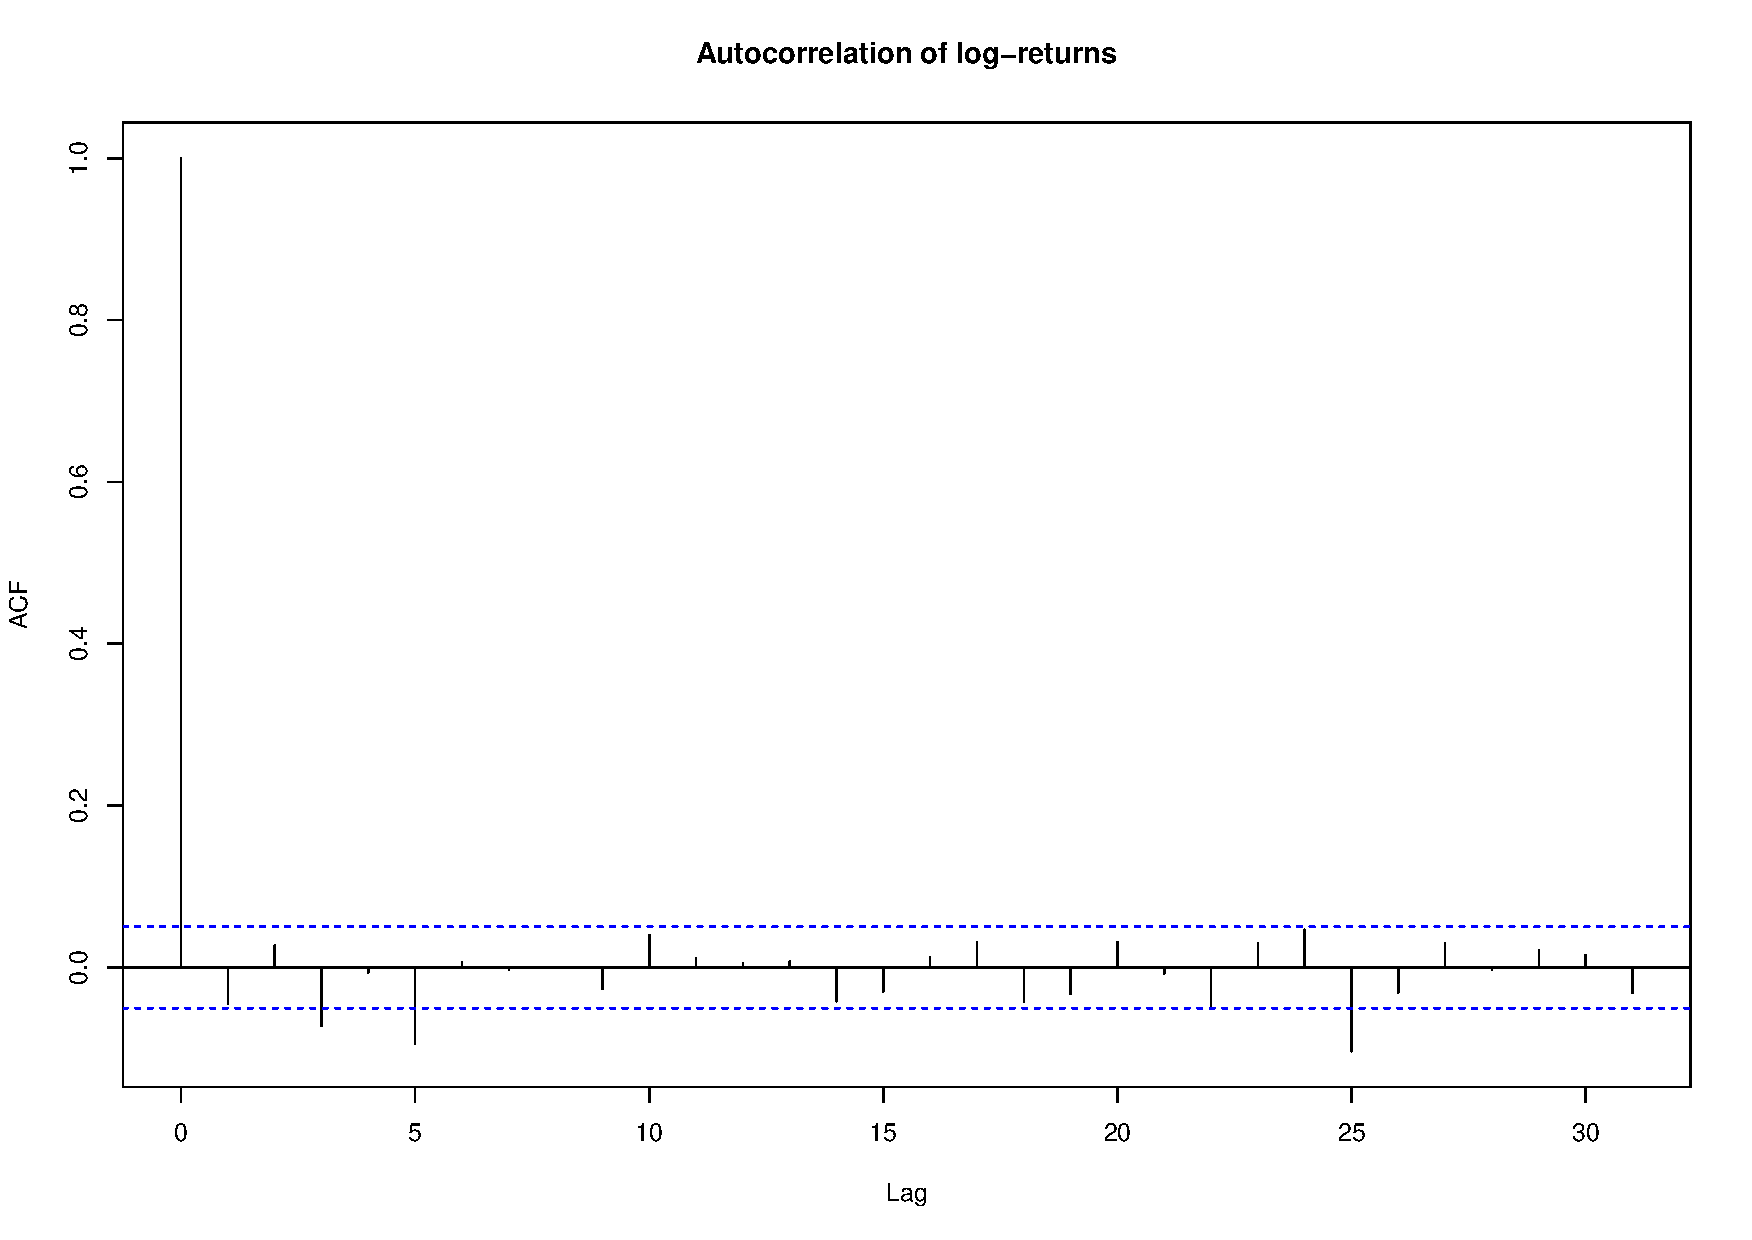
\includegraphics[scale=0.35]{img/finData/acfDailyLogRet}
	\caption{Autocorrelations of daily S\&P500 log-returns}
	\label{fig:acfDailyLogRet}
\end{figure}

Figure \ref{fig:HistLogRet} shows the histogram for daily, weekly and 
monthly log-returns of the S\&P500. It has been introduced with the 
intention of illustrating stylized facts 2 and 4. It clearly shows the heavy 
tails and how it evolves towards a normal distribution as the returns time 
scale increases.\\

\begin{figure}[hbtp]
	\centering
	\begin{subfigure}{.5\textwidth}
		\centering
		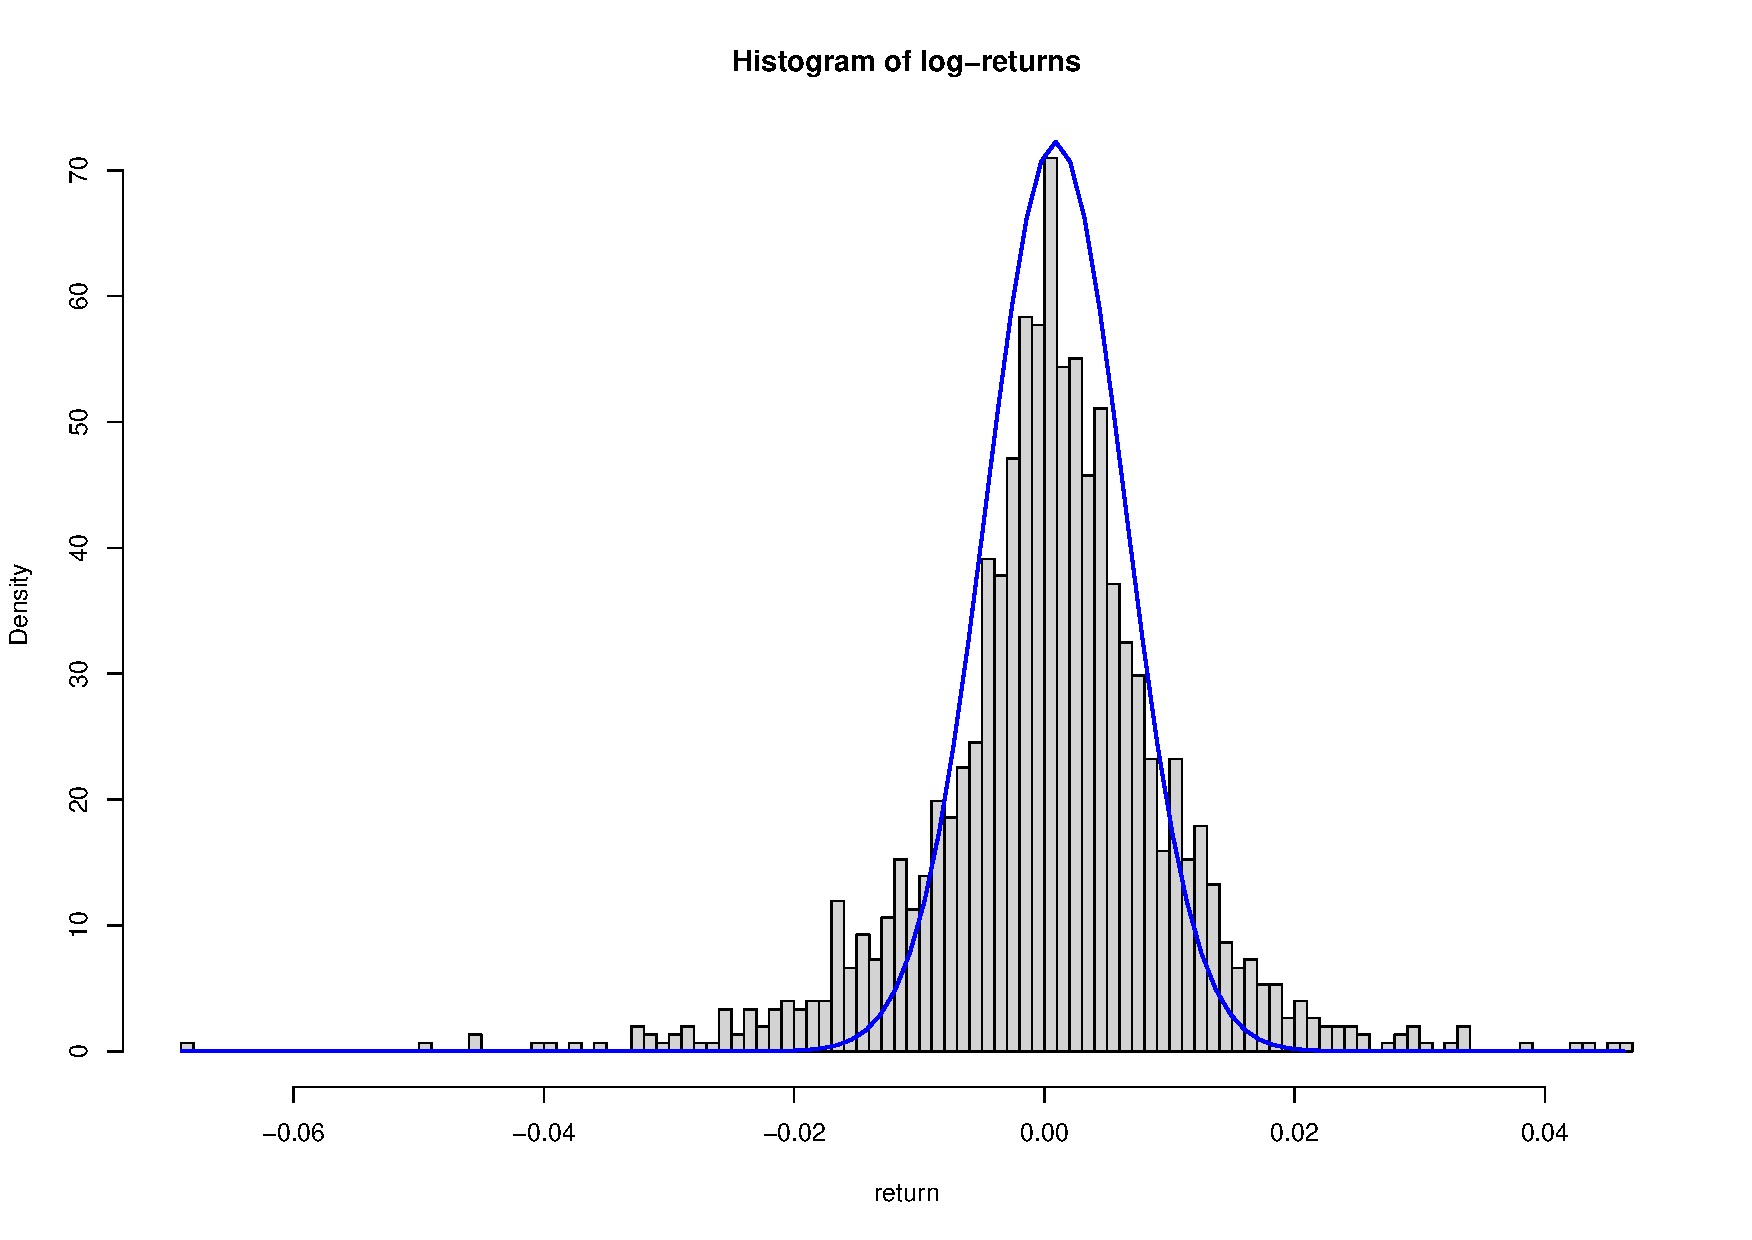
\includegraphics[scale=.2]{img/finData/histDailyLogRet}
		\caption{Daily log-returns}
	\end{subfigure}%
	\begin{subfigure}{.5\textwidth}
		\centering
		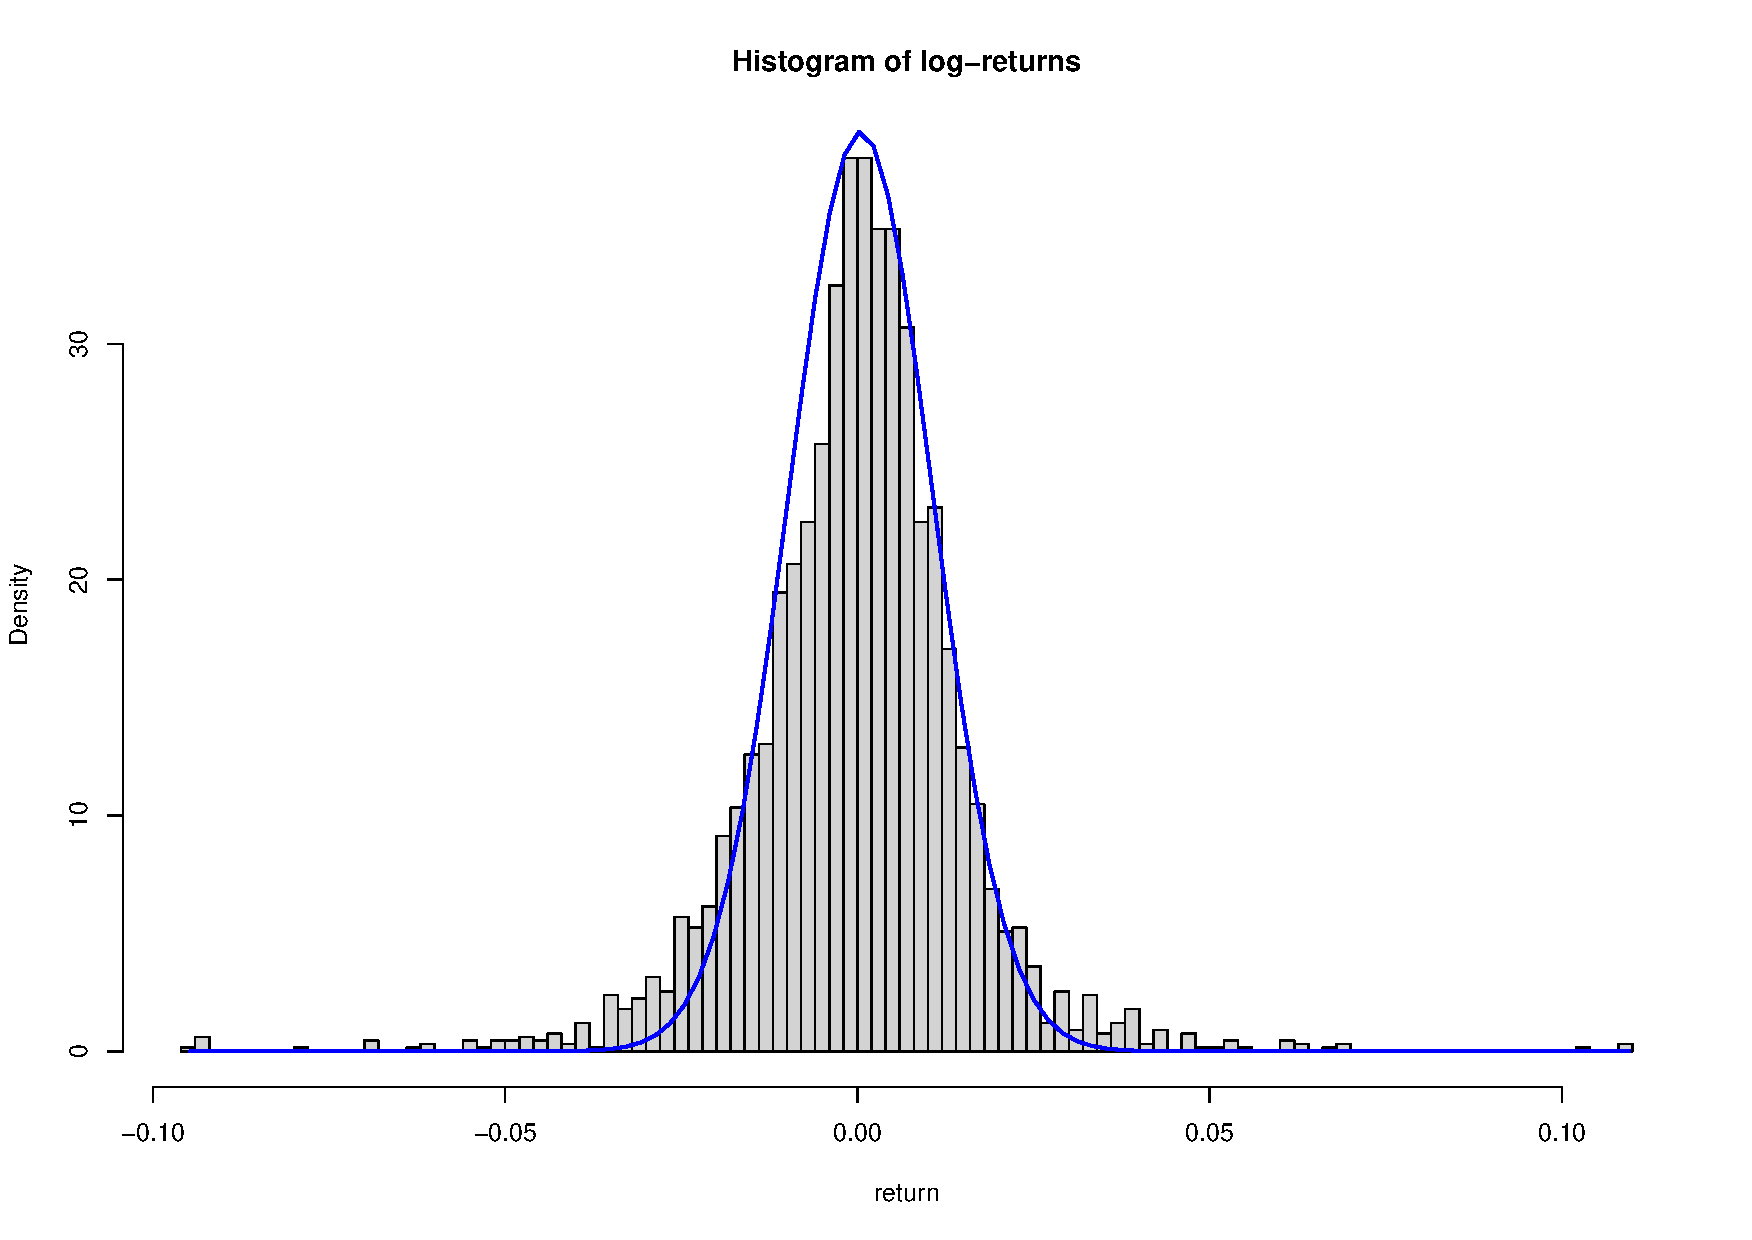
\includegraphics[scale=.2]{img/finData/histWeeklyLogRet}
		\caption{Weekly log-returns}
	\end{subfigure}
	
	\vspace{.4cm}
	
	\begin{subfigure}{\textwidth}
		\centering
		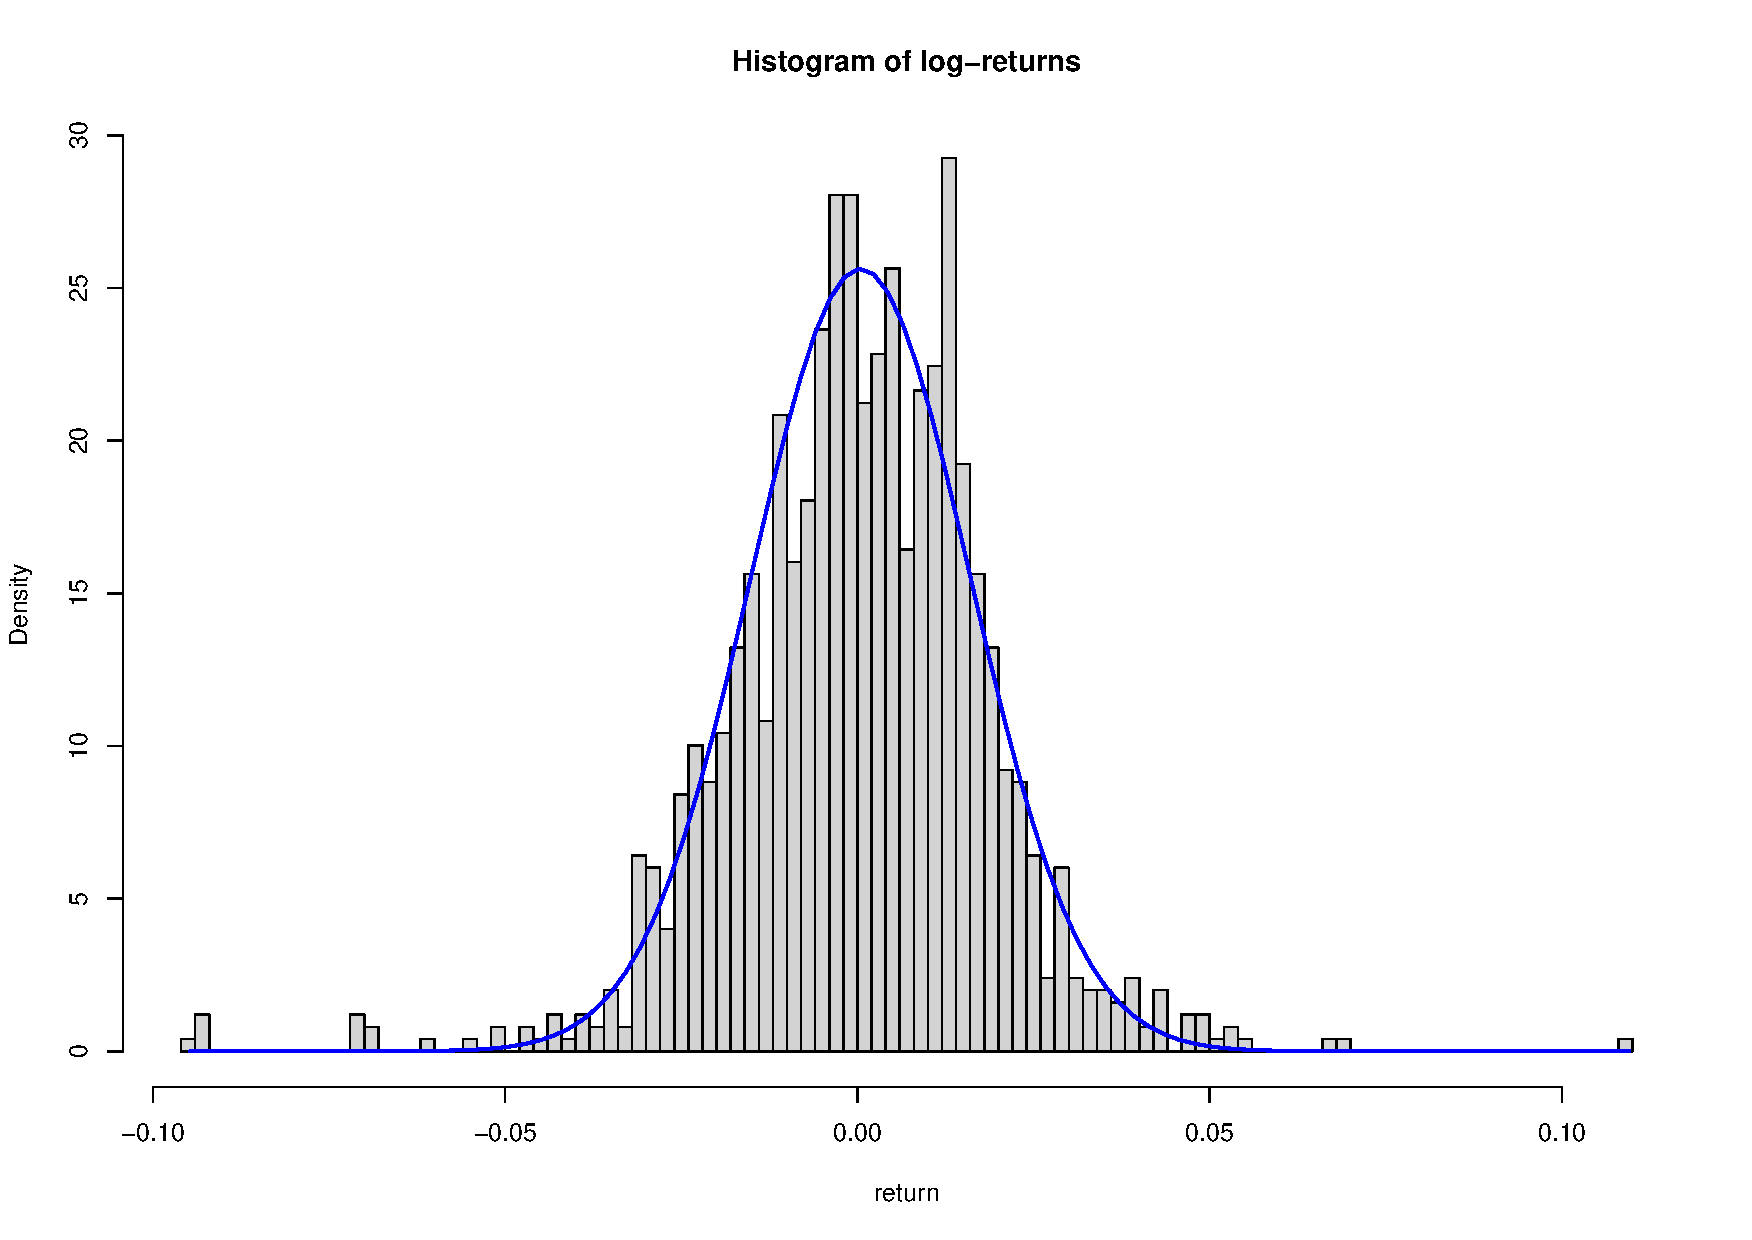
\includegraphics[scale=.2]{img/finData/histMonthlyLogRet}
		\caption{Monthly log-returns}
	\end{subfigure}
	
	\caption{Pdf fitted to S\&P500 log-returns}
	\label{fig:HistLogRet}
\end{figure}

Lastly, figure \ref{fig:QQPlotLogRet} illustrates, via QQ (Quantile 
Quantile) plots, that log-returns do not follow a normal distribution. 
Beforehand, it is pertinent to introduce special notation for quantiles:
given a r.v. X, a \textbf{quantile} $q_\alpha$ is a real number s.t. $P(X 
\leq q_\alpha) = \alpha$\\

That said, Quantile Quantile plots order the observations, and then map them 
to the graph such that the value of the x-axis is the equivalent quantile of 
$Z \sim N(0,1)$, and the value of the y-axis is the quantile of the sample. 
That way, if one wants to test if $X \sim N(\mu, \sigma^2)$, then knowing 
that the quantiles would just be shifted and/or scaled, the corresponding QQ 
Plot should be a line.\\

In the case of the S\&P500 log-returns (see figure \ref{fig:QQPlotLogRet}), 
the QQ Plots are not lines, implying that log-returns are not Normal. In 
addition, the curvature at the extremes is a clear sign of a heavy-tailed 
distribution.

\begin{figure}[hbtp]
	\centering
	\begin{subfigure}{.5\textwidth}
		\centering
		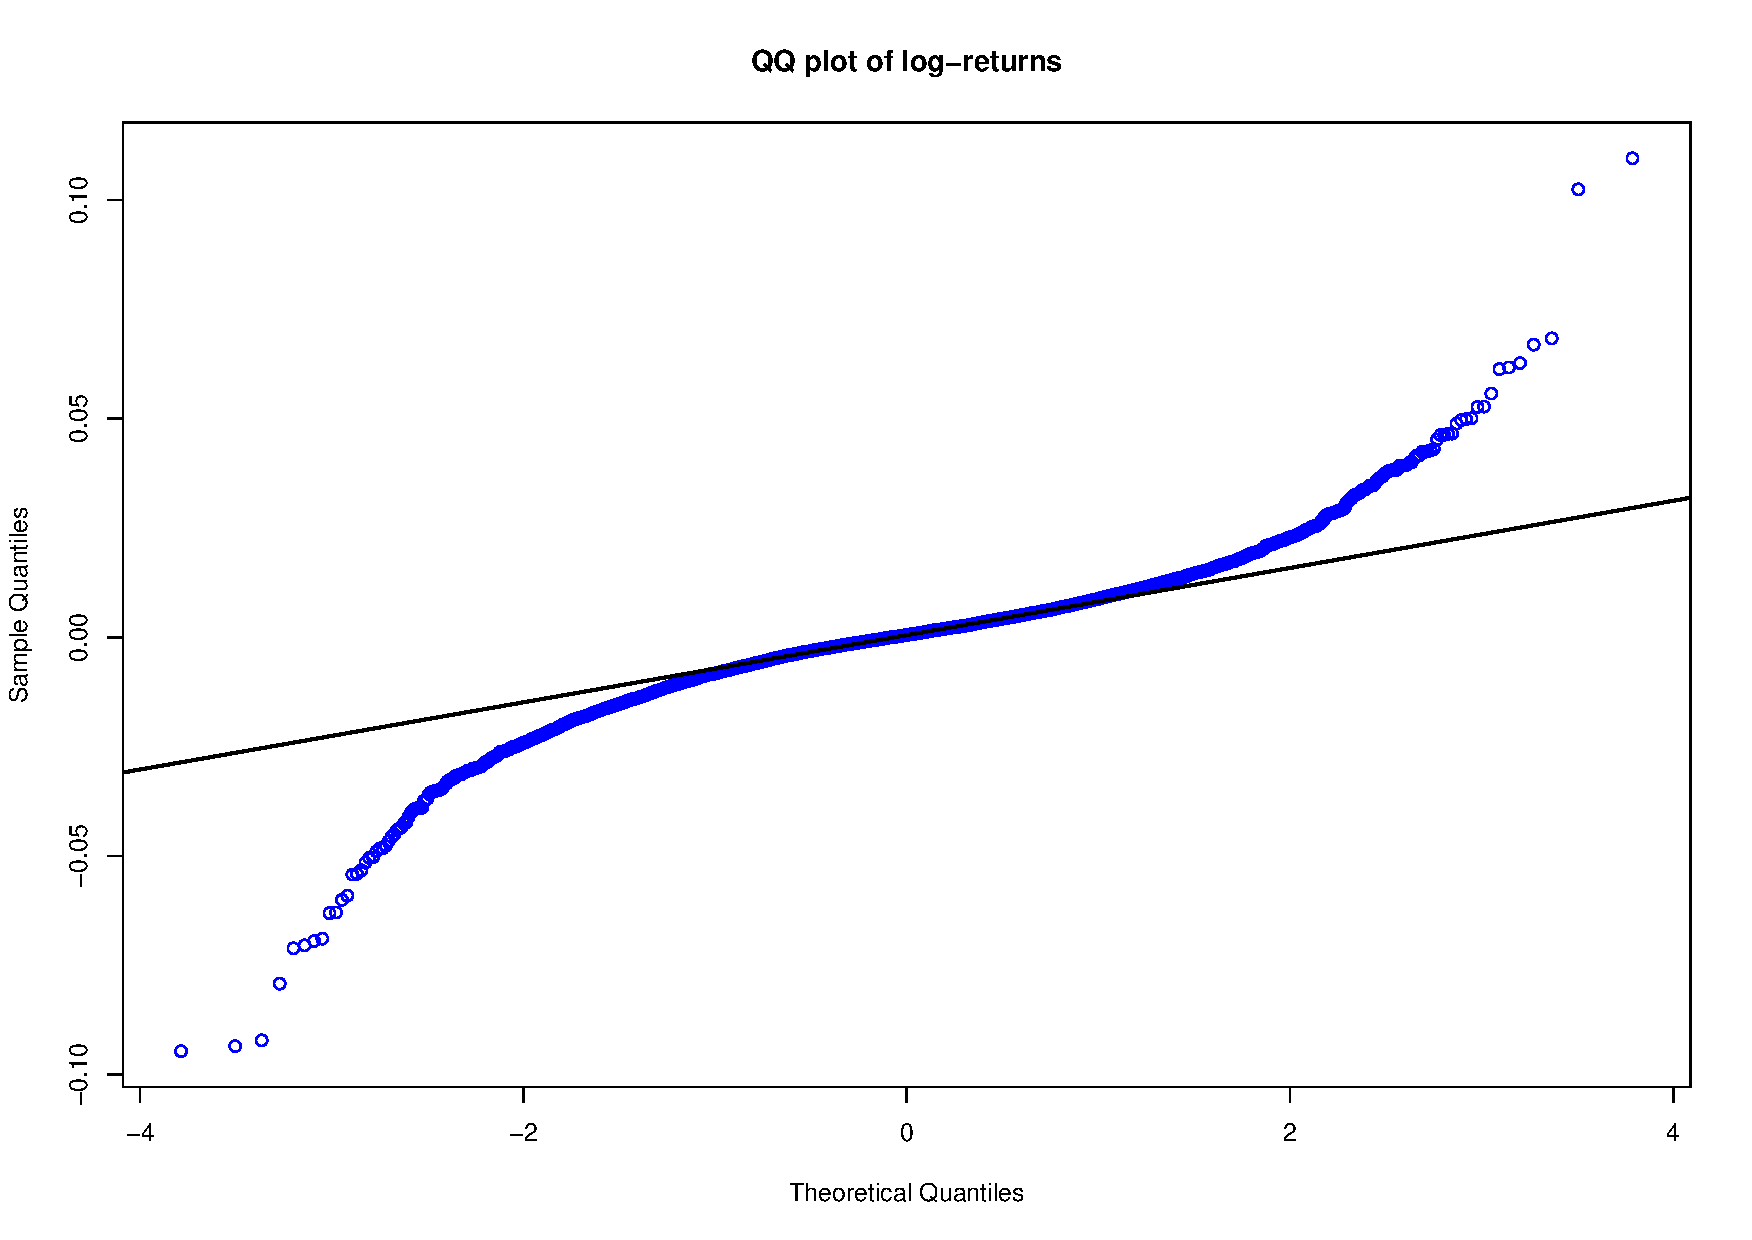
\includegraphics[scale=.2]{img/finData/QQPlotDailyLogRet}
		\caption{Daily log-returns}
	\end{subfigure}%
	\begin{subfigure}{.5\textwidth}
		\centering
		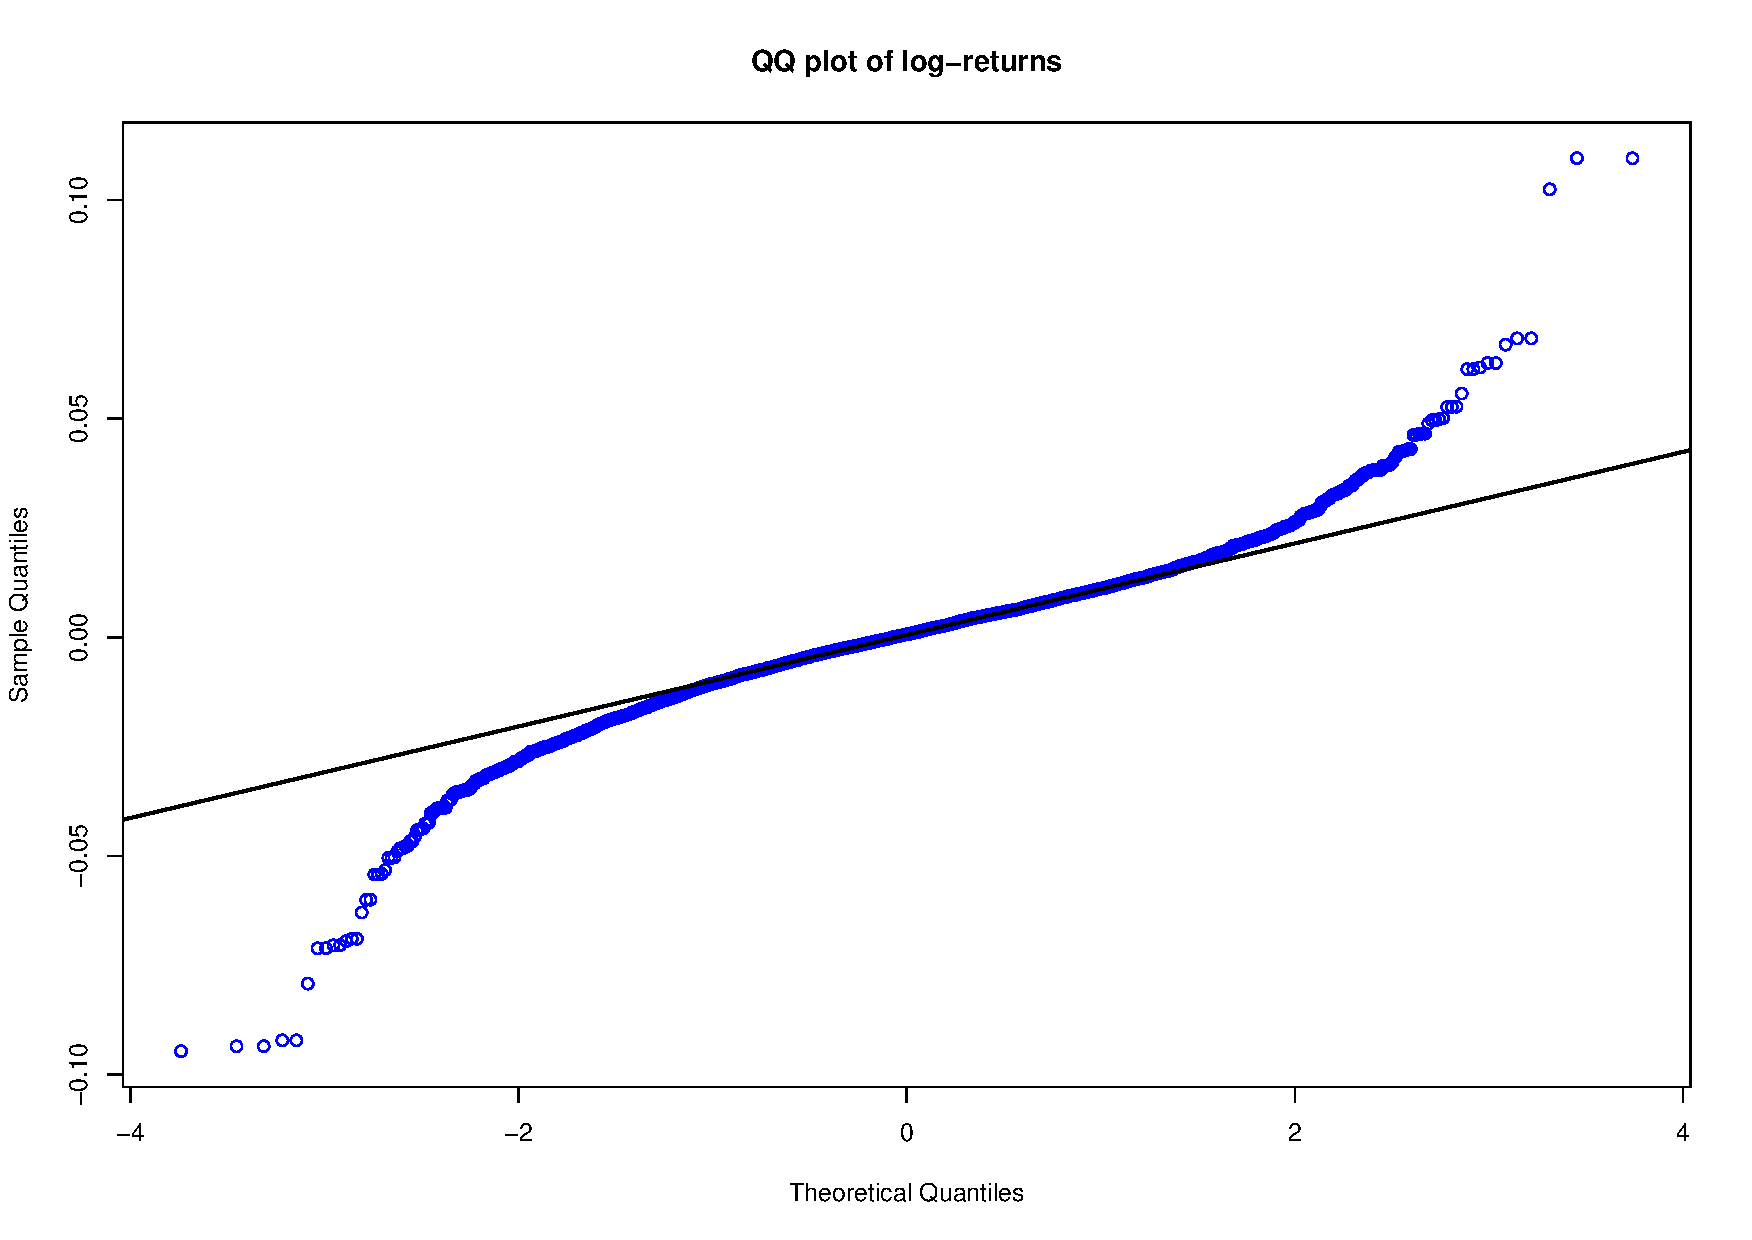
\includegraphics[scale=.2]{img/finData/QQPlotWeeklyLogRet}
		\caption{Weekly log-returns}
	\end{subfigure}%
	
	\vspace{.4cm}
	
	\begin{subfigure}{\textwidth}
		\centering
		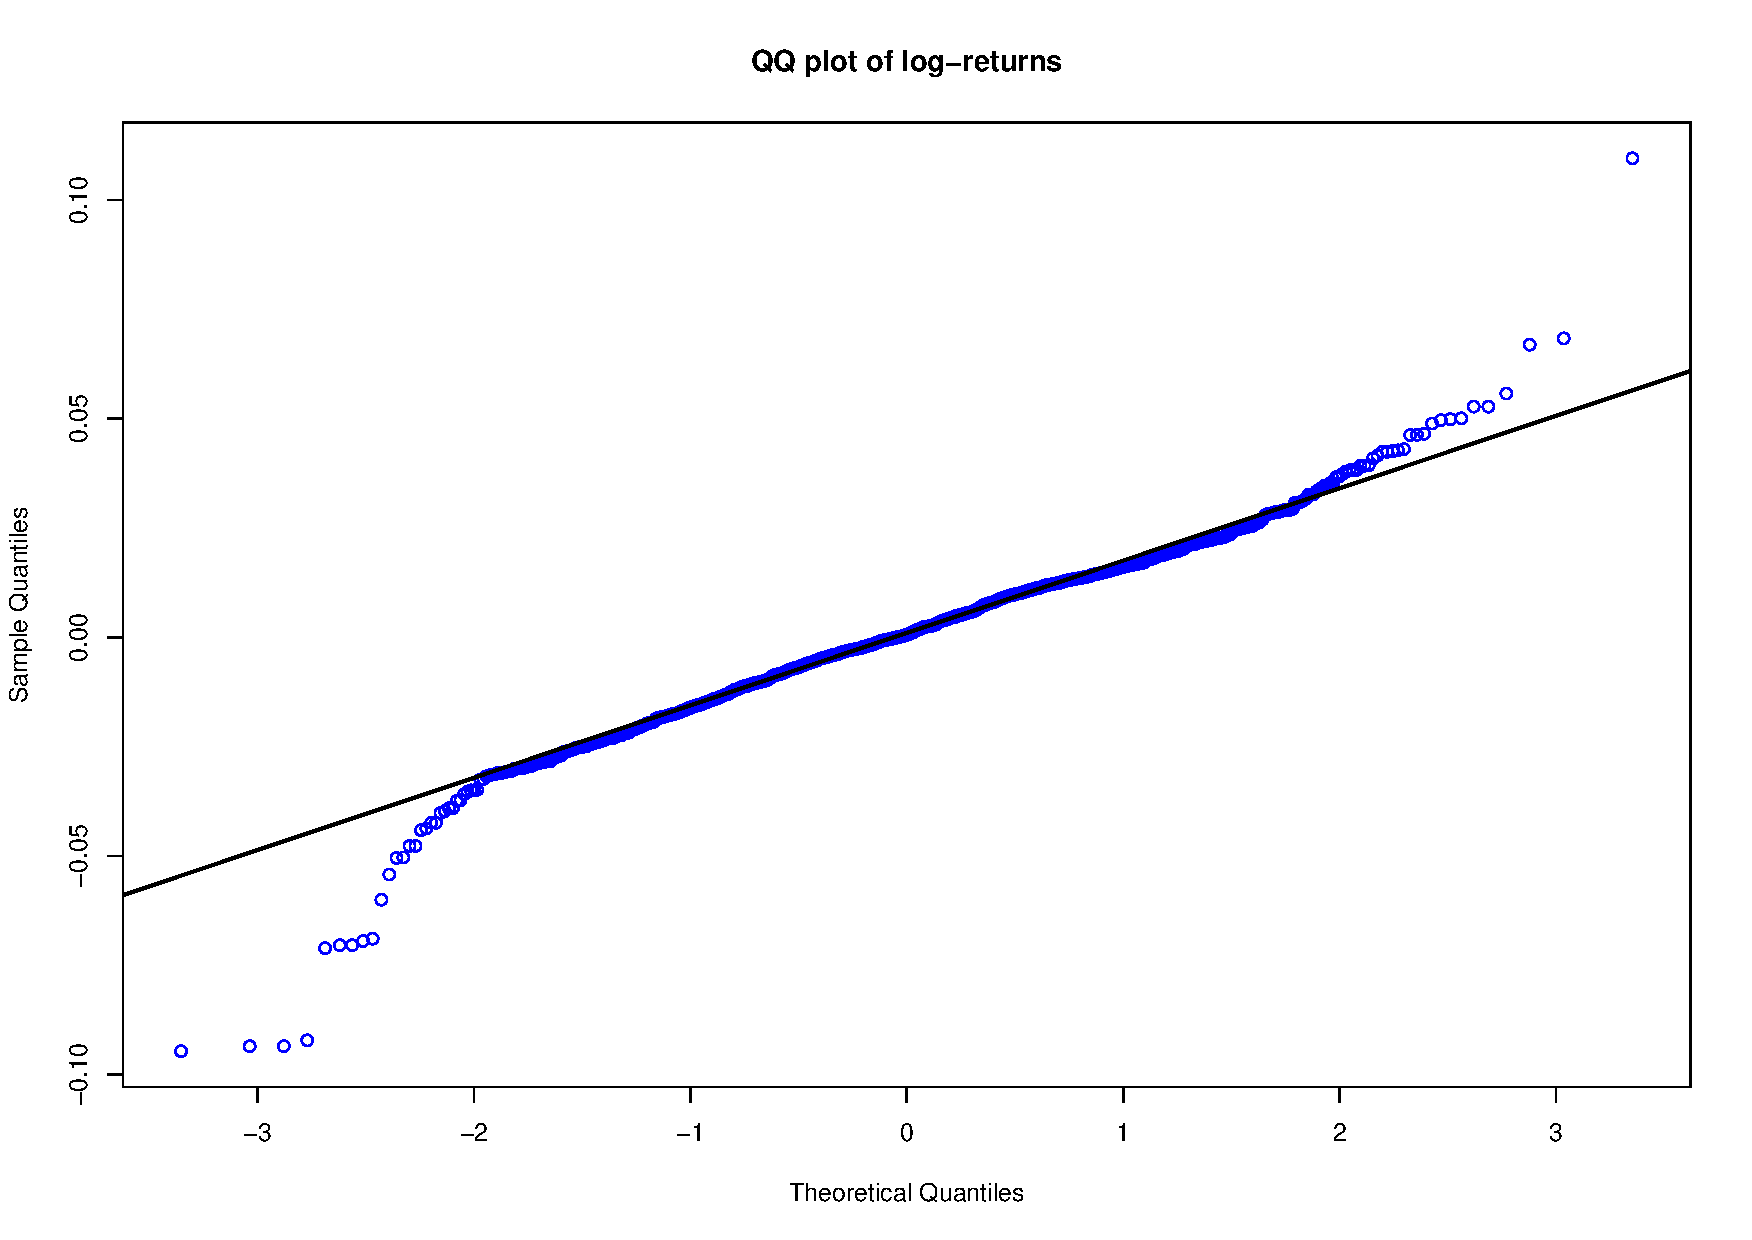
\includegraphics[scale=.2]{img/finData/QQPlotMonthlyLogRet}
		\caption{Monthly log-returns}
	\end{subfigure}
	
	\caption{QQ Plots of S\&P500 log-returns}
	\label{fig:QQPlotLogRet}
\end{figure}

\newpage

\section{Portfolios}
This section will introduce the concept of portfolios, which essentially 
means that one can allocate a certain budget to different financial products 
instead of buying a single asset. In this work, $N$ will represent the 
number of securities and $\mathbf{w} \in \mathbb{R}^N$ the vector of weights 
assigned to each asset. Accordingly, the price of each stock considered in 
the portfolio will be noted as $p_t^i$, where $i \in \{1,\ \ldots ,\ N\}$.\\

Regarding notation for portfolio returns it is useful to set the following 
terms:
\begin{itemize}
	\item \textbf{Money available (budget):} $B$
	
	\item \textbf{Portfolio linear returns:}  $R_t^P$
	
	\item \textbf{Portfolio log-returns:} $r_t^P$
	
	\item \textbf{Linear returns of asset $i$}: $R_t^i \longleftrightarrow
	\textbf{R}_t = [ R_t^1 ,\ \ldots ,\ R_t^N ]$
	
	\item \textbf{Log-returns of asset $i$}: $r_t^i \longleftrightarrow 
	\textbf{r}_t = [ r_t^1 ,\ \ldots ,\ r_t^N ]$
\end{itemize}

Recognizing that the amount of money invested in asset $i$ is simply 
$B w_i$, $R_t^P$ can be computed as:
\begin{align*}
	R_t^P = \frac{\sum_{i = 1}^{N} B w_i \cdot (1 + R_{t}^{i})}{B} - 1 =
	\sum_{i = 1}^{N} (w_i + w_i \cdot R_{t}^{i}) - 1 =
	\textbf{w} \cdot \textbf{R}_{t}\\
	r_t^P = \log (1 + R_t^P)\hfill
\end{align*}

Where it has been used that:
\begin{itemize}
	\item $\sum_{i=1}^N w_i = 1$ because in the cases that are going to be 
	considered there is no leverage. This constraint just means that the sum 
	of the money invested in each asset is $B$
	
	\item If $B w_i$ is the initial wealth of asset $i$ at time $t-1$, then 
	the final wealth is $B w_i \cdot (1 + R_t^i) = B w_i \cdot 
	\frac{p_t^i}{p_{t-1}^{i}}$
\end{itemize}

\section{Long and short positions}
When opening a position it is really important to distinguish between long
and short positions. A long position (or going long on some stock) is the 
most common way to invest since it just means that you buy an asset and you 
sell it at some point, expecting to earn a return.\\

On the contrary, if you short a stock, you first sell a stock that someone 
has lent you and then try to repurchase it at a lower price to return the 
stock to the lender. That way, if the stock goes down in price, you would 
earn a profit by selling high and buying low.\\

The following examples will attempt to clarify what was mentioned before:
\subsection*{Long position}
Suppose the prices of stock \textbf{ABC} at times $t_0$ and $t_1 := t_0 + 1$ 
are $p_{t_0} = 100\$ $ and $p_{t_1} = 115\$ $ respectively. Then, the return 
is: $R_{t_1} = \frac{115}{100} - 1 = 0.15$. If at $t_0$ one buys 10 stocks 
of \textbf{ABC} at market value ($B = 10 \cdot p_{t_0} = 1000\$ $), the end 
wealth at $t_1$ will be $B \cdot (1 + R_{t_1}) = 1150\$ $. Thus, the final 
profit has been 150\$.\\

Conversely, if the stock would have gone down in price at time $t_1$, money 
would have been lost. At this point, it is obvious that long positions will 
only be profitable if the stock price ends at a higher value than the one 
when the position was opened.

\subsection*{Short position}
Following the example of the long position, suppose that at time $t_0$ one 
shorts 10 stocks of \textbf{ABC}. That means that 10 stocks will be lent to 
us to be sold immediately at market value, making one hold 1000\$ in cash.\\

As the stock at time $t_1$ has gone up in value, one repurchases the shares 
at 1150\$, realizing a 150\$ loss. However, if at time $t_1$ the stock price 
would have been $p_{t_1} = 85\$ $, then the stocks would have been 
repurchased at 850\$, realizing a 150\$ profit. From a practical standpoint, 
the end wealth of a short position can be calculated as 
$B \cdot (1 - R_{t_1})$ since:

\begin{equation*}
	R_{t_1}^{\text{short}} = \frac{\text{profits}}{p_{t_0}} =  
	\frac{p_{t_0} - p_{t_1}}{p_{t_0}} = - R_{t_1}
\end{equation*}

where \textbf{profits} means the money you would earn if you shorted one 
stock (selling at $p_{t_0}$ and buying at $p_{t_1}$) and 
$R_{t_1}^{\text{short}}$ the return realized at $t_1$ by shorting one stock 
at $t_1$.\\

As a final note, it should be pointed out that shorting a stock can lead to 
ever-growing losses. This is caused by the definition of shorting, which 
implies receiving stocks from someone who expects them back. So if a stock 
keeps going up in price, then the stocks will be repurchased at a price that 
will keep growing. On the other hand, if one goes long on a stock, the 
maximum capital that can be lost is the initial one, which would only happen 
if the stock price went to 0.

\section{Financial Metrics}
In this section, a series of financial metrics will be shown so as to 
compare results in the succeeding chapters:
\begin{itemize}
	\item Sharpe Ratio
	\item Information Ratio
	\item Drawdown
\end{itemize}

\subsection*{Sharpe Ratio}
The Sharpe ratio is extremely useful since it allows to compare assets 
independent of the returns and variability. This metric, as defined by 
William F. Sharpe in \cite{sharpe1994sharpe}, was introduced with the
concept of reward per unit of variability in mind:
\begin{equation}
	\label{eqn:williamFSharpe}
	\text{SR} = \frac{\mathbb{E}[R_t - r_f]}{\sqrt{\text{Var}[R_t - r_f]}}
\end{equation}

The term $r_f$ in equation \ref{eqn:williamFSharpe} is the risk-free return, 
which is the rate of return you can achieve with zero risk. An example of 
this is the 1 month U.S. Treasury bills. As a side note, the term $r_f$ was 
introduced because assets carrying risk must surpass $r_f$ to encourage 
investors to buy them.

\subsection*{Information Ratio}
Similarly to the Sharpe Ratio, the Information Ratio is useful to compare 
the returns achieved with a benchmark:

\begin{equation*}
	\label{eqn:informationRatio}
	\text{IR} = \frac{\mathbb{E}[R_t - R_b]}{\sqrt{\text{Var}[R_t - R_b]}}
\end{equation*}
Where $R_b$ are the returns of the benchmark, $\alpha := \mathbb{E}[R_t - 
R_b]$ is the excess return, and $\sqrt{\text{Var}[R_t - R_b]}$ is one of the 
many definitions of tracking error.

\subsection*{Drawdown}
The drawdown of an investment at time $t$ is noted as $D(t)$ and is a 
risk-related metric that measures the relative drop from a historical peak 
(High Water Mark):
\begin{equation*}
	D(t) = \frac{\text{HWM}(t) - p_t}{\text{HWM}(t)}
\end{equation*}

Where 

\begin{equation*}
	\text{HWM}(t) = \max_{1 \leq \tau \leq t} p_t
\end{equation*}

\section{High Frequency Data}
\label{sec:highFrequencyData}
The purest form of financial data is called tick data, which collects the 
information of sellers and buyers of a financial product. The way traders 
enter the market is by posting \textbf{orders}, that can be either 
\textbf{buy or sell orders}. A buy (sell) order represents the will of a 
trader to buy (sell) $m$ units of an asset at a price $p$.\\

Before giving an overview of tick data, a few concepts should be defined:
\begin{itemize}
	\item \textbf{Bid price} ($b_t$): maximum price out of all the buy 
	orders at time $t$.
	
	\item \textbf{Ask price} ($a_t$): minimum price out of all the sell 
	orders at time $t$.
	
	\item \textbf{Mid price:} $m_t = \frac{a_t + b_t}{2}$
	
	%\item \textbf{Price:} ($p_t$) price of the last asset sold.
	
	%\item \textbf{Volume:} ($v_t$) number of stocks exchanged.
	
	\item \textbf{Tick size:} smallest change in price a stock can move 
	(e.g. 0.001\$).
\end{itemize}

Note that orders are ordered in price and time. This means that if one posts 
an order to sell 10 units of an asset at time \textbf{10:00:21} at a price 
of 10.00\$, then one would have less priority than a person that wanted to 
sell 4 units at time \textbf{10:00:18} at the same price.\\

Having said that, a few remarks follow:
\begin{enumerate}
	\item If one were to buy or sell \textbf{one unit} of an asset, it could 
	be done instantly at prices $a_t$ and $b_t$ respectively.

	\item If the tick size did not exist then traders could jump ahead by 
	increasing the bid or ask prices by a small amount $\epsilon$.
	
	\item The spread ($a_t - b_t > 0$) is a measure of the liquidity of the 
	asset in question. That is, how buyers and sellers agree.
	
	\item Data is \textbf{inhomogenous} in the sense that it does not arrive 
	at fixed time intervals (see table \ref{tab:tickData}). In fact, only 
	when agreements are made between buyers and sellers will a new tick be 
	recorded. Therefore, in a period of high activity a lot of 
	\textbf{ticks} ($\{t, p_t, b_t, a_t, v_t \}$) will be recorded in a 
	short time span, and vice versa.
\end{enumerate}


\begin{table}[htbp]
\caption{Example of tick data}
\label{tab:tickData}
\centering
\begin{tabular}{ |C{5cm}|C{2cm}|C{2cm}|C{2cm}|C{2cm}| }
	\hline
	$t$ & $p_t$ & $b_t$ & $a_t$ & $v_t$\\
	\hline
	2013-01-02 08:00:00 & 67.18 & 67.18 & 67.78 & 125\\
	2013-01-02 08:12:56 & 67.70 & 67.19 & 67.70 & 125\\
	2013-01-02 08:12:56 & 67.75 & 67.75 & 67.82 & 125\\
	2013-01-02 08:47:15 & 67.91 & 67.21 & 67.93 & 150\\
	2013-01-02 09:29:09 & 67.55 & 67.52 & 67.55 & 200\\
	2013-01-02 09:29:09 & 67.56 & 67.51 & 67.57 & 200\\
	2013-01-02 09:29:10 & 67.56 & 67.51 & 67.58 & 200\\
	2013-01-02 09:29:10 & 67.58 & 67.51 & 67.57 & 100\\
	2013-01-02 09:29:10 & 67.58 & 67.52 & 67.58 & 100\\
	2013-01-02 09:29:11 & 67.57 & 67.52 & 67.58 & 200\\
	\hline
\end{tabular}
\end{table}
